%!TEX root = rapport.tex

\subsection{Sift algorithm variations}
\label{sec:sifting}
As described in Section~\ref{sec:heap:sifting}, two different strategies for sifting have been implemented. A memory efficient using less than $V$ space that reads/writes backwards and a version that uses up to $2V$ space but only reads/writes forwards.

We choose to do a small experiment for our fastest streams with the two sifting implementations, as we were unsure about the penalty (if any) obtained by doing I/O backwards.

For the BufferedStream, the two algorithms were benchmarked for different node sizes and buffer sizes. In all performed experiments, ranging from a buffer size of 4 kB to 256 kB and node size ranging from 2 MB to 8 MB it was found that memory efficient sifting was always superior. We believe this is due to:

\begin{itemize}
\item Buffers and caches, since they are always filled by reading forward.
\item The memory inefficient algorithm interleaves operations on the two streams, where the memory efficient algorithm only uses one stream at a time. For example in the memory inefficient implementation, when the elements of the two nodes are merged into internal memory, elements are read from both of the streams, and even though the streams are buffered, the disk must seek from one part of the disk to another when the buffers needs to be refilled. This is not the case for the memory efficient implementation.
\end{itemize}

For the memory mapped stream, a similar experiment was done. Figure~\ref{fig:m-efficiency} shows the result of this experiment. As can be seen, the memory inefficient algorithm is the fastest for small node sizes, whereas the memory efficient algorithm is faster for large node sizes.

Like before, the stream interleaving done by the memory inefficient algorithm is believed to be contributing to this: For small node sizes it does not matter that much, because relatively few elements are read and most of them can be cached, while for larger node sizes the disk will begin reading from two different areas. To make things worse, the memory inefficient algorithm uses about twice the amount of memory for doing the merge, yielding less space for the operating system to use for caching of the memory mapped file. Therefore, when using a large node size, more pages of the memory mapped file may be swapped to disk, resulting in cache misses later in the test execution.

\begin{figure}
  \centering
  \includegraphics[width=1\columnwidth]{m_efficiency}
  \caption{Comparison of memory inefficient and memory efficient sifting algorithm, when using MMapStream with varying node sizes and 1 GB of elements.}
  \label{fig:m-efficiency}
\end{figure}

\subsection{Parameter weeding}
As described in Section~\ref{sec:implementation:parameters}, the implemented heap has a lot of adjustable parameters which all may have an influence on its performance. In order to limit the time needed for running experiments, the parameter space has been weeded out, such that it does not include obviously bad settings.

We have only considered settings of parameters satisfying the following constraints:
\begin{equation}
  \label{eqn:memory}
  \underbrace{V}_{\textrm{Sifting}} + \underbrace{2P \ceil*{\frac{N}{V}}}_{\textrm{Caching}} + \underbrace{(d + 1)B}_{\mathclap{\substack{
  \textrm{Refill for}\\\textrm{buffered streams}
  }}} \leq M
\end{equation}
\begin{equation}
  \label{eqn:dvn}
  dV\leq N
\end{equation}
Constraint~\ref{eqn:memory} says that all buffers and caches used by the heap should fit into main memory. If this was not the case, memory trashing would occur, resulting in more I/Os than anticipated. Note that for the memory mapped stream there is no explicit buffer, hence when the inequality in \eqref{eqn:memory} is tight, no space is left for the operating system to cache files opened with memory mapping.

Assume a fixed node size, then the performance of sifting improves when the height $h = \log_d{\frac{N}{V}}$ of the tree is decreased because the recursion of sifting ends after fewer iterations. During refilling, $d+1$ streams are open, hence when using a buffered stream $d+1$ buffers are allocated. Therefore, $d$ can be increased as long as the buffers fit into memory.

All configurations not satisfying \eqref{eqn:dvn} will have the same result as $d=\frac{N}{V}$. Moreover parameter values have been increased by a factor of $2$.

\subsection{Streams}
In this section the different streams will be benchmarked and compared.

\subsubsection{Cached stream}
We found that the cached stream improves the performance of the BufferedStream, FStream and SysStream. For SysStream the improvement is expected, since it has no buffer or cache on its own. For the BufferedStream and FStream, a speedup was found with a very small cache size, with decreasing performance when increasing the cache size. We believe this is due to the cache is "conflicting" with the buffers of the underlying streams, but using a very small cache helps when doing the refill operation, since this eliminates the first read from every child node where none or only few elements are are taken.

Figure~\ref{fig:m-cache-size-comparison} shows that MMapStream performs significantly worse when using an extra level of cache. Moreover, the size of the cache does not seem to have a any significant effect on the running time. This is believed to be because that the operating system handles the caching of the memory mapped file itself, and hence adding an extra layer of cache is redundant, and introduces overhead and possibly interferes with the cache strategy employed by the operating system.

\begin{figure}
  \centering
  \includegraphics[width=1\columnwidth]{m_cache_size_comparison}
  \caption{Comparison of the running time for different node sizes using different cache sizes for MMapStream.}
  \label{fig:m-cache-size-comparison}
\end{figure}

In the following experiments, a small cache of 128 elements are used for BufferedStream, FStream and SysStream, whereas no cache is used for MMapStream.

\subsubsection{SysStream and FStream}
By experimenting, we have found that SysStream and FStream performs worse for all tested parameter combinations. Therefore, we have chosen to exclude these streams from all subsequent comparisons.

The reason for the SysStream being slow, is due to its lack of buffering to reduce the number of I/Os. For FStream a buffer is added, however, we found that it was dominated by BufferedStream even with the same buffer size. This is also to be expected, since the buffers used in BufferedStream are optimized for the specific application of an external heap, whereas this is not the case for the more generic FStream.

\subsection{MMapStream}
As seen in figure~\ref{fig:m-efficiency} in section~\ref{sec:sifting}, the node size resulting in the fastest running time for sorting 1 GB of elements is 4 MB. Therefore we have chosen to use this node size when running benchmarks of MMapStream.

From figure~\ref{fig:m:vary-d} it can be seen that a bigger value of $d$ improves running time. Hence, when running benchmarks, we have chosen to make $d$ as large as possible. 

\begin{figure}[h!]
  \centering
  \includegraphics[width=1\columnwidth]{m_d}
  \caption{Running time of MMapStream when varying the $d$ parameter.}
  \label{fig:m:vary-d}
\end{figure}

However, when sorting very big input sizes, the $d$ value can not be increased arbitrary because at least one page from every node should be able to fit the memory mapped file cache, otherwise a lot of trashing would occur. There are two possible solutions to this problem:
\begin{itemize}
\item Increase the node size. This is only possible up to the main memory size, otherwise sifting will begin to put its internal buffer on disk.
\item Restrict $d$ such that there is memory left for the operating system to use as cache when doing refill.
\end{itemize}
Both of the solutions will result in decreased performance, and the latter of the solutions would result in more I/Os, but ultimately this is unavoidable because of the I/O sorting lower bound.

For all the benchmarked input sizes, it has always been possible to simply increase $d$ such that the resulting heap was of height 2.

\subsection{BufferedStream}

\begin{figure}[h!]
  \centering
  \includegraphics[width=1\columnwidth]{b_final.pdf}
  \caption{Time for sorting a 1 GB file varying the buffer size (x-axis) and the node size (series)}
  \label{fig:b_final}
\end{figure}

As can be seen in figure~\ref{fig:b_final}, the best performing configuration for buffered stream sorting 1 GB elements is a 32 kB buffer size and a node size of 4 MB. Larger block sizes forces $d$ to be smaller which figure~\ref{fig:m:vary-d} shows hurts performance. But 4 MB node size is also faster than 2 MB node size. We believe this is due to the fact that a larger node size yields more sequential read/write that buffered streams are especially suited for. When the node size increases, the best buffer size also increases. Having a larger buffer size means more sequential reads/writes and higher performance when utilized properly.

Another interesting observation from the figure is that the configurations (except for a node size of 32 MB) begins to perform worse at a point when using larger buffer sizes. This effect is especially visible for a node size of 2 MB. We believe this is due to underutilized buffers. For instance, consider a refill using a node size of 2 MB, $d=512$ and a 32 kB buffer. The algorithm potentially refills $\frac{V}{2}=\frac{\textrm{2 MB}}{2}$ elements and assuming an equal number of elements from each child is moved up, $\frac{V}{2d}=\frac{\textrm{2 MB}}{2 \cdot 512}=\textrm{2 kB}$ elements from each child is used which is significantly less than the buffer size of each child. A similar argument can be used for sifting where a smaller portion is sifted upwards when $d$ is larger and therefore, the buffer is again potentially underutilized.

From this point on, a node size of 4 MB and a buffer size of 32 kB is used when comparing against other other streams.

\subsection{Comparison}

\begin{figure}
  \centering
  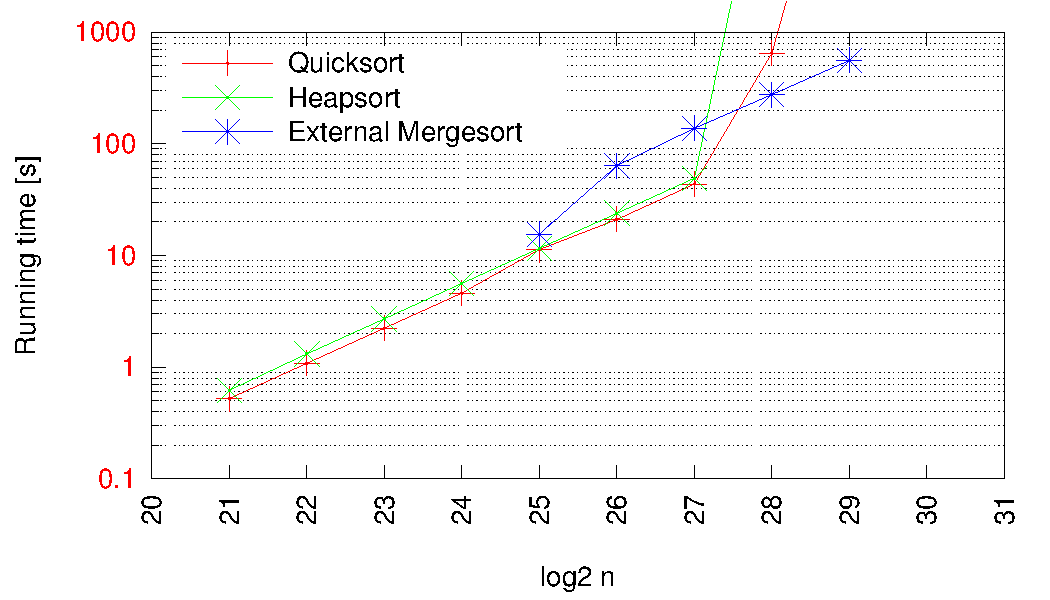
\includegraphics[width=1\columnwidth]{best_sort}
  \caption{Ratio between external mergesort and other sorting algorithms.}
  \label{fig:best_sort}
\end{figure}

We have chosen to omit SysStream and FStream in this comparison because they are inferior to BufferedStream and MMapStream.

Figure~\ref{fig:best_sort} shows how heap sorting using the external heap with BufferedStream and MMapStream compares to external mergesort as implemented in project 1 and in-memory quicksort. It can be seen that the external heapsort is slower than external mergesort with both MMapStream and BufferedStream. This is in agreement with the findings in R. Fadel et. al. \citep{Fadel1999345}.

It seems that the ratio between external heapsort and external mergesort gets worse for larger input sizes. This is not expected since both solutions satisfies the optimal sorting I/O bound. However, note that:
\begin{itemize}
\item In project 1 we saw that the number of input scans in external mergesort was given by the height of the merge tree. For the external heapsort the effect of the tree height is not as profound since the height of the tree does not directly relate to the number of input scans.
\item The number of refill operations is linear in the input size and each refill operation does not only induce a constant number of I/Os when $d$ increases. We may see a more constant ratio if the node size was increased as the input size got larger.
\end{itemize}
Therefore, when an extra level is added to the merge tree, we would expect a drop in the ratio between external mergesort and external heapsort. The reason no drop is seen in the plot is that for the tested input sizes the merge tree always had height 2.

The plot also shows that BufferedStream is approximately 50\% \\ slower than MMapStream. This is opposed to what we found in the external mergesort. We believe this is due to a more random access pattern in the external heapsort which memory mapped files are especially good at due to its least-recently-used cache strategy.